
\section{Wer vertritt wen?}
\label{vertretung}

Es gibt zwei Arten von Gremien, die im Folgenden vorgestellt werden: Einerseits gibt es studentische Gremien (Fachschaftsräte, Studierendenrat), in denen nur Studenten vertreten sind. Andererseits gibt es universitäre Gremien (Fakultätsräte, Senat), in denen Professoren, wissenschaftliche Mitarbeiter, nichtwissenschaftliche Mitarbeiter und Studierende gemeinsam vertreten sind.
%Eine Übersicht über die Gremien ist in Abbildung \ref{fig:gremien} auf Seite \pageref{fig:gremien} gegeben.

\begin{figure}[htb]
    \centering
    %Hier kommt eine Tikz Picture hin und kein odg Ding zwecks kompatibilität und Sexyness
    %\includegraphics[width=\textwidth]{Bilder/studentische_gremien.odg}\\
    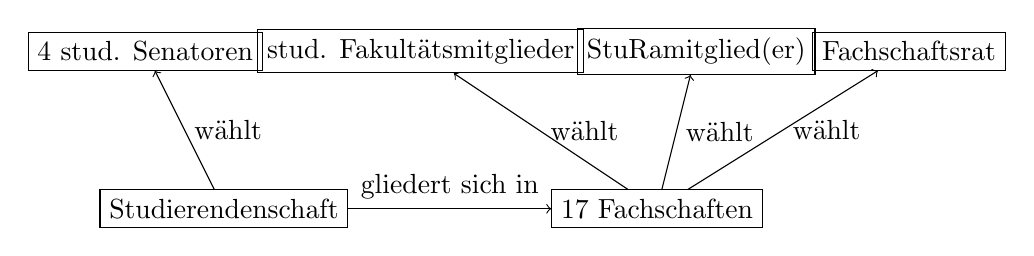
\begin{tikzpicture}
    \node[draw] (Senatoren) at (0,0) {4 stud. Senatoren};
    \node[draw] (Fakultaetsmitglieder) at (3.5,0) {stud. Fakultätsmitglieder};
    \node[draw] (StuRa) at (7,0) {StuRamitglied(er)};
    \node[draw] (FSR) at (9.7,0) {Fachschaftsrat};
    \node[draw] (Studis) at (1,-2) {Studierendenschaft};
    \node[draw] (FS) at (6.5,-2) {17 Fachschaften};
	%
  	\path (Studis) -- (FS) node[midway, above] {gliedert sich in};
  	\draw[->,draw] (Studis) to (FS);
  	%
  	\path (Studis) -- (Senatoren) node[midway, right] {wählt};
  	\draw[->,draw] (Studis) to (Senatoren);
  	%
  	\path (FS) -- (Fakultaetsmitglieder) node[midway, right] {wählt};
  	\draw[->,draw] (FS) to (Fakultaetsmitglieder);
  	%
  	\path (FS) -- (StuRa) node[midway, right] {wählt};
  	\draw[->,draw] (FS) to (StuRa);
  	%
  	\path (FS) -- (FSR) node[midway, right] {wählt};
  	\draw[->,draw] (FS) to (FSR);
    \end{tikzpicture}
    \caption{Übersicht über die studentischen Gremien}
    \label{fig:gremien}
\end{figure}

\subsection{Fachschaftsräte}

\begin{figure}[h]
    \centering
    
\includegraphics[scale=0.36]{fsrsw}
    \caption{hinten: Maximilian Büttner, Norman Holtz, René-Pierre Geiß, Florian Lücke vorne: Steffen Manigk, Florian Johnke, Felix Schmidt}
             \label{fig:fsr}
\end{figure}

\begin{table}[!h]
    \centering
    \begin{tabular}{llll}
        \toprule
        \textbf{Sprecher} & Florian Lücke & Master Informatik & 3.~Sem.\\
                 & \multicolumn{3}{l}{\email{florian.luecke@fsr-matheinfo.de}}\\
        \midrule
        \textbf{Stellvertreter} & Florian Johnke & Lehramt Mathematik, & 3.~Sem.\\
                                && Lehramt Informatik & 3.~Sem.\\
                       & \multicolumn{3}{l}{\email{florian.johnke@fsr-matheinfo.de}}\\
        \midrule
        \textbf{Finanzer~I} & Steffen Manigk & Lehramt Mathematik  & 7.~Sem.\\
                   & \multicolumn{3}{l}{\email{steffen.manigk@fsr-matheinfo.de}}\\
        \midrule
        \textbf{Finanzer~II}  & Norman Holtz & Bachelor Wirtschafts- & 5.~Sem.\\
                              && mathematik\\
                     & \multicolumn{3}{l}{\email{norman.holtz@fsr-matheinfo.de}}\\
        \midrule
                     & Felix schmidt & Master Informatik & 3.~Sem.\\
                     & \multicolumn{3}{l}{\email{felix.schmidt@fsr-matheinfo.de}}\\
        \midrule
                     & Maximilian Büttner & Bachelor Mathematik & 5.~Sem.\\
                     & \multicolumn{3}{l}{\email{maximilian.buettner@fsr-matheinfo.de}}\\
        \midrule
                     & René-Pierre Geiß & Bachelor Mathematik, & 3.~Sem.\\
                     && Bachelor Bioinformatik & 5.~Sem.\\
                     & \multicolumn{3}{l}{\email{rene.geiss@fsr-matheinfo.de}}\\
        \bottomrule
    \end{tabular}
    \caption{Mitglieder des Fachschaftsrats 2014/15}
\end{table}
\newpage
Der Fachschaftsrat ist die Interessenvertretung der Studentinnen und Studenten eines Fachbereichs und besteht in unserem Fall aus sieben Mitgliedern, welche jedes Jahr im Mai neu gewählt werden.
Er ist unter anderem dazu da, den Kontakt zu den Professoren und Mitarbeitern zu halten.
Wenn also Fragen und Probleme jeglicher Art auftreten, habt keine Scheu, sondern wendet euch an uns.
Wir versuchen dann gemeinsam eine Lösung zu finden.

Außerdem organisiert der Fachschaftsrat Feiern, damit bei dem vielen Stress des Studiums der Spaß nicht verloren geht.
Da wären unter anderem das alljährliche Sommerfest, die Weihnachtsfeier und die Erstsemesterparty.
Diese Veranstaltungen sind für die Mitglieder der Fachschaft -- also für euch.
Eintrittspreise habt ihr also nicht zu erwarten und Getränke und Grillgut sind sehr günstig.
Ihr findet detaillierte Infos weiter hinten im Heft.

Der Fachschaftsrat finanziert sich aus einem Teil der \EUR{6,10}, die ihr jedes Semester als Studierendenbeitrag bezahlt.
Schließlich ist der Fachschaftsrat ein Teil des Studierendenrates.
Wenn ihr eine Idee haben solltet, was man für die Fachschaft tun oder kaufen könnte, so versuchen wir es gerne zu finanzieren.
Gleiches gilt für besondere Aufgaben, die eigentlich nicht zum Studium gehören (\;z.B. Programmierwettbewerbe, Seminare, \ldots).

Wenn ihr später einmal selbst den Studierenden des Fachbereichs helfen wollt, lasst euch einfach bei der nächsten Wahl im Frühling aufstellen.

\web{http://fachschaft.mathinf.uni-halle.de}\\
\email{fachschaft@mathinf.uni-halle.de}

\subsection{Studierendenrat}

Ähnlich wie der Fachschaftsrat (FSR) die Interessen einer Fachschaft vertritt, setzt sich der Studierendenrat (StuRa) für die Belange der gesamten Studierendenschaft ein.
Die Aufgaben der beiden Gremien sind dabei verschieden.
Im Gegensatz zum FSR ist der StuRa für universitätsweite und allgemeine Angelegenheiten zuständig.
Zum Einen diskutiert der StuRa über hochschulpolitische Themen,  vertritt die Studierenden gegenüber der Universität und Land und verwaltet die Studierendenschaftsgelder, zum Anderen bietet er verschiedene Service-Leistungen an, unterstützt die verschiedensten Projekte finanziell (jeder kann einen solchen Projektantrag stellen) und bietet eine kostenlose Rechtsberatung, die bei Rechtsschwierigkeiten von jedem Studierenden in Anspruch genommen werden kann, Sozialberatung und Bafög-Beratung an.
Sogar zinslose Sozialdarlehen kann der Studierendenrat bewilligen.

Der Studierendenrat trifft sich in der Vorlesungszeit in der Regel zweiwöchentlich.
Bei diesen Sitzungen wird viel diskutiert und über verschiedenste Anträge abgestimmt, jeder kann dabei sein und Anträge stellen.
Zur Organisation der anfallenden Arbeit wählt der StuRa Sprecher:

\begin{itemize}
    \item Vorsitzende des Sprecherkollegiums, die die Arbeit des StuRa koordinieren und den StuRa nach Außen vertreten.
    \item Sitzungsleitende Sprecher, die die Sitzungen des StuRa organisieren, an denen Anträge an den StuRa eingereicht werden und die dazu Sprechstunden anbieten.
    \item Sprecher für Finanzen, die sich um korrekte Abrechnungen und den Haushaltsplan kümmern.
    \item Sprecher für Soziales, die Sozialanträge behandeln, und bei Fragen rund um BAföG, Wohngeld, GEZ, Stipendien, Krankenkasse, Versicherung, Studieren mit Kind usw. euch zur Seite stehen,
    \item einen Senatssprecher (siehe \ref{senat} Senat)
    \item einen Fachschaftskoordinator, der die Koordination und den Austausch unter den Fachschaftsräten leitet
\end{itemize}

Alle Sprecher bilden gemeinsam das Sprecherkollegium.
Daneben gibt es diverse Ausschüsse und Arbeitskreise (z.B. den AK Studierende mit Kind oder die Interessenvertretung Lehramt).
In Arbeitskreisen kann jeder Studierende mitwirken bzw. solche gründen.
Eine aktuelle Auflistung aller Arbeitskreise befindet sich auf der Website des StuRa.
Die Mitglieder des Studierendenrates werden - wie der FSR - von den Studierenden, also euch, direkt gewählt.
Dabei kandidiert ein Studierender immer in seiner jeweiligen Fachschaft, also nicht auf universitätsweiten Listen.
Die Fachschaft Mathematik/Informatik ist eine sehr kleine.
Daher haben wir auch nur eines der 35 Mandate im StuRa.


\web{www.stura.uni-halle.de}\\
\email{stura@uni-halle.de}\\

\subsection{Fakultätsräte}

Die Fakultätsräte setzen sich aus Mitgliedern der Gruppe der Hochschullehrer, Vertretern der Studierenden, des akademischen Mittelbaus sowie der technischen Angestellten zusammen.
Die Institute Mathematik und Informatik können jeweils einen studentischen Vertreter in ihren Fakultätsrat schicken.
Dabei gehört die Mathematik in die Naturwissenschaftliche Fakultät II und die Informatik in die Naturwissenschaftliche Fakultät III.
Aufgabe ist die Entscheidung über die Mittelverwendung und über Fragen der Forschung und Lehre an der jeweiligen Fakultät.
Dazu gehört u.a. die Beschlussfassung der Studien- und Prüfungsordnung.
Außerdem ist der Fakultätsrat für die Erteilung akademischer Grade und Titel zuständig und auch für die Wahl des Vertreters der Fakultät, den Dekan.
Somit sind die Entscheidungen, die dort getroffen werden, für die Studenten eher von mittel- und langfristiger Bedeutung.

Jedoch sind Vorschläge, wie das Studium aus eurer Sicht hier zu verbessern ist, sehr willkommen.
Wir als studentische Vertreter werden auf jeden Fall von unserem Stimm- und Rederecht Gebrauch machen, falls ihr Vorschläge habt.

Ihr könnt euch mit jedem Problem an den Fachschaftsrat wenden, der eure Anliegen gegebenenfalls natürlich auch in den Fakultätsrat weiterleitet.

\web{http://www.natfak3.uni-halle.de/fakultaetsrat/}\\
\email{fachschaft@mathinf.uni-halle.de}\\


\subsection{Senat}
\label{senat}

Der Senat ist das zentrale Beschlussfassungsorgan der Hochschule.
Er bestimmt den Unihaushalt, beschließt Richtungsentscheidungen der Uni, beschließt die Einrichtung und Schließung von Studiengängen, beschließt die Berufungen von Professoren und muss die von den Fakultätsräten beschlossenen Prüfungsordnungen u.Ä. genehmigen.
Stimmberechtigte Mitglieder im Senat sind 12 Professorinnen bzw. Professoren, vier Studierende, vier wissenschaftliche MitarbeiterInnen und zwei sonstige MitarbeiterInnen.
Die vier studentischen Vertreter könnt ihr bei den Hochschulwahlen auf uniweiten Listen wählen.
Die Dekane sind beratende Mitglieder, ebenso wie der durch den Studierendenrat gewählte Senatssprecher und der Kanzler.

Der Senat bildet Kommissionen zur Vorbereitung und Beratung von Entscheidungen.
Zurzeit gibt es vier Kommissionen, die sich verschiedenen Themenbereichen widmen:

\begin{itemize}
    \item Studium und Lehre
    \item Forschung
    \item Haushalt und Struktur
    \item Berufungsprüfungskommission
\end{itemize}

In jeder Kommission wirken bis zu 3 Studierende mit.
Sie werden von den studentischen Senatoren im Senat vorgeschlagen und vom Senat bestätigt.
In der Regel schreibt der Studierendenrat zu Beginn des Studienjahres die Mitarbeit in den Kommissionen aus.
Dann kann sich jeder Studierende melden und wird zu einem Gespräch in den Studierendenrat eingeladen.

\link{http://verwaltung.uni-halle.de/senat\_der\_verwaltung/}

